% % \chapter*{\centering{\large{LEMBAR PENGESAHAN}}}
% % \thispagestyle{empty} {\bf }Dengan ini saya mahasiswa Fakultas
% % Matematika dan Ilmu Pengetahuan Alam, Universitas Negeri Jakarta

% % \vskip3mm

% % \begin{tabular}{ll}
% %   Nama & : Ci \\
% %   No. Registrasi & : 1313619007 \\
% %   Program Studi & : Ilmu Komputer \\
% %   Judul & : Pengembangan Aplikasi Math Braille Translator \\ & \hspace{0.2cm} Berbasis Android Menggunakan Acuan Simbol Braille \\ & \hspace{0.2cm} Matematika Indonesia Revisi Tahun 2011
% % %  Judul & : Pengaruh Penggunaan \emph{Color Model} LAB dan HLS dalam \\ & \hspace{0.2cm} Kalibrasi Warna Luka Menggunakan Metode Segmentasi \\ & \hspace{0.2cm} \emph{K-Means} dan \emph{Mean Shift}\\
% % \end{tabular}

% % \vskip3mm

% % \noindent \hskip10mm Menyatakan bahwa proposal ini telah siap diajukan untuk sidang pra skripsi.
% % %\begin{center}
% % %Menyatakan bahwa skripsi ini telah siap diajukan untuk sidang skripsi.
% % %\end{center}

% % \begin{center}
% % \vskip3mm

% % Menyetujui,

% % \vskip3mm
% % \begin{spacing}{1.25}

% % \begin{tabular}{ccc}
% %   \hskip-2mm Dosen Pembimbing I & \qquad \qquad \qquad \qquad & \hskip-6mm Dosen Pembimbing II \\
% %    &  &  \\
% %    &  &  \\
% %    &  &  \\
% %    &  &  \\
% %   \hskip-2mm \underline{\textbf{Muhammad Eka Suryana, M.Kom.}} &  & \hskip-6mm \underline{\textbf{Ari Hendarno, S.Pd., M.Kom.}} \\
% %   \hskip-2mm NIP. 19851223 201212 1 002 &  & \hskip-6mm NIP. 19881102 202203 1 002 \\
% % \end{tabular}
% % \end{spacing}
% % \end{center}
% % \vskip3mm
% % \begin{center}
% % Mengetahui, \\
% % Koordinator Program Studi Ilmu Komputer
% % \end{center}
% % \begin{spacing}{1.25}
% % { \ }
% % \\
% % \\
% % { \ }\begin{center}
% % \underline{\textbf{Dr. Ria Arafiyah, M.Si.}} \\
% % {NIP. 19751121 200501 2 004}
% % \end{center}
% % \end{spacing} 
% 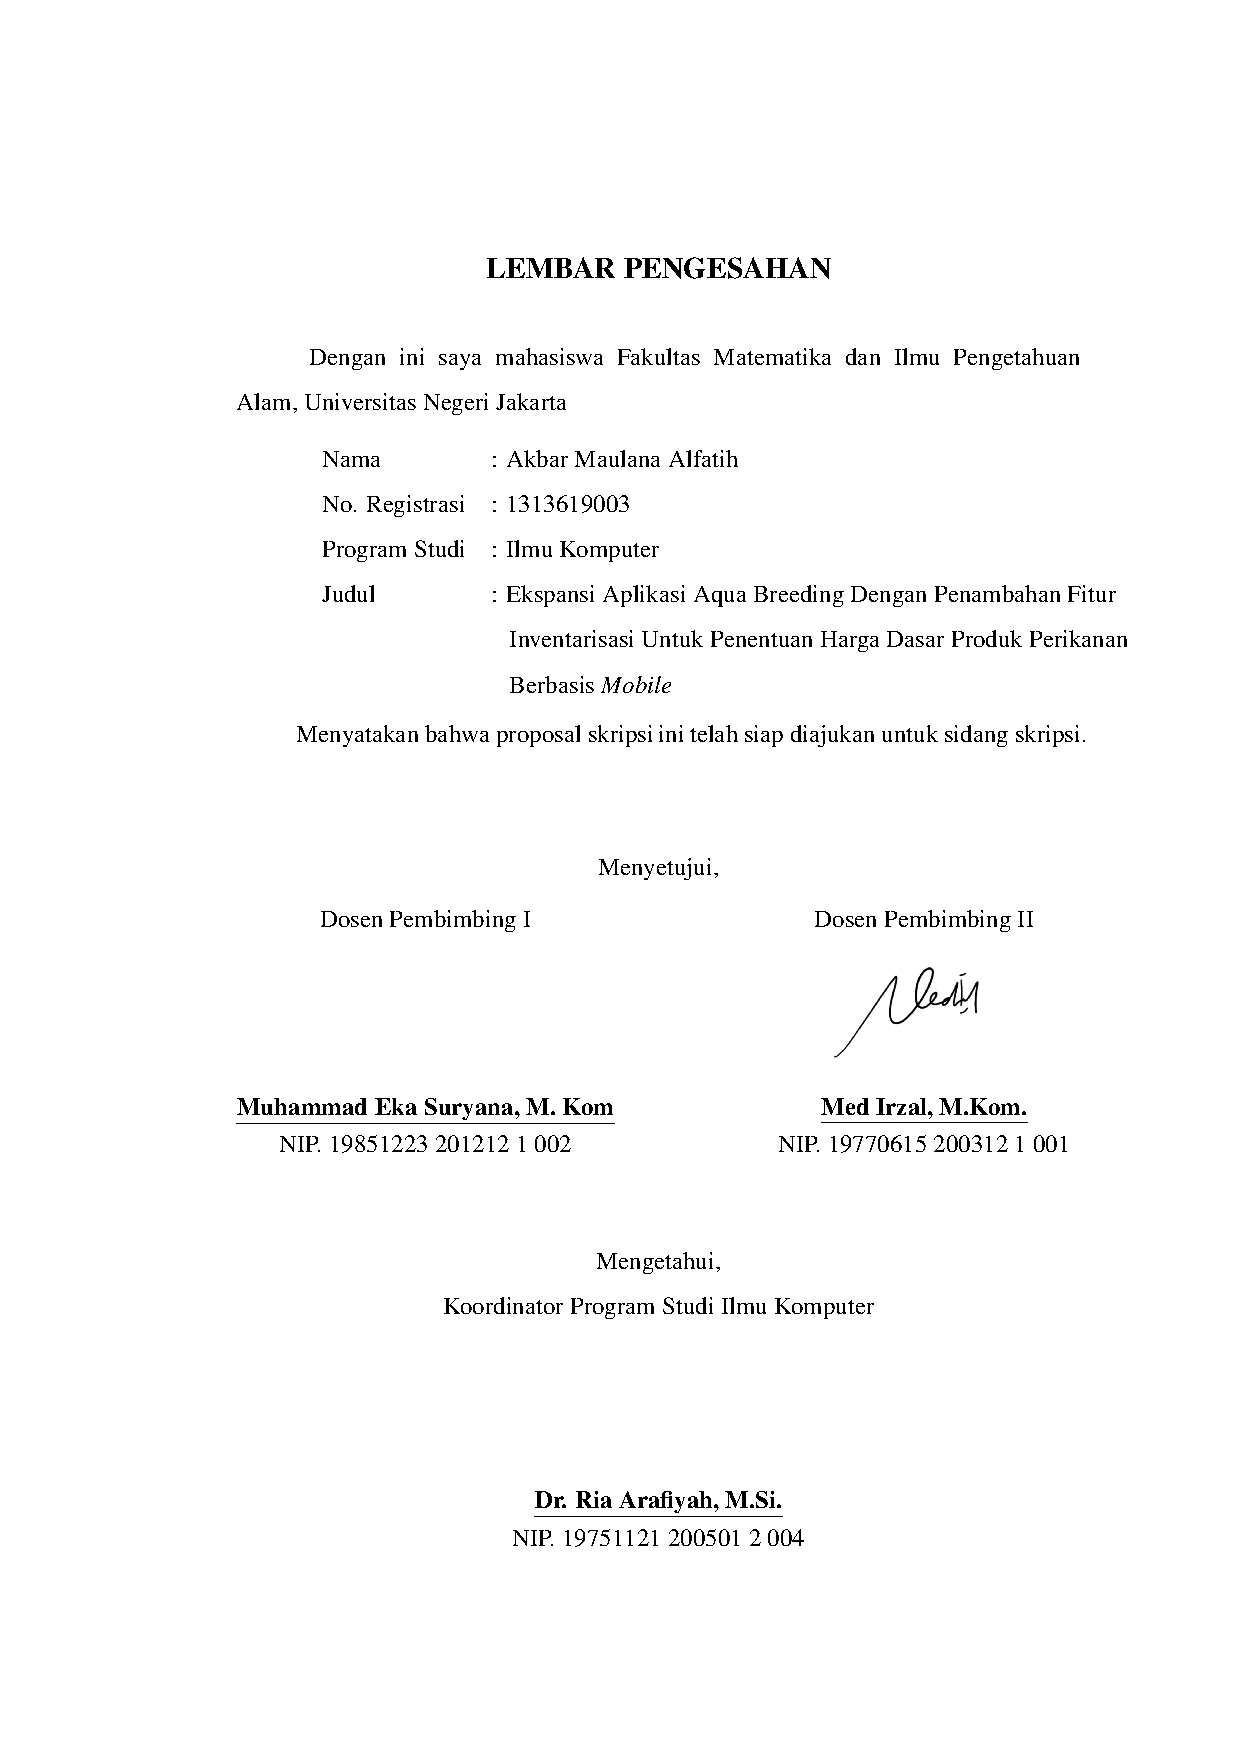
\includepdf[pagecommand={\thispagestyle{plain}},
%   pages=1]{assets/lembar_pengesahan_skripsi.pdf}